\chapter{VBTE}
Følgende afsnit beskriver VBTE'ens hardware i de enkelte blokke, grænsefladerne derimellem samt funktionen af blokkene.

\section{Overordnet design}
Nedenfor ses det overordnede hardware blokdiagram. Herefter følger en beskrivelse af de forskellige blokke samt signaler.
\begin{figure}[H]
\centering
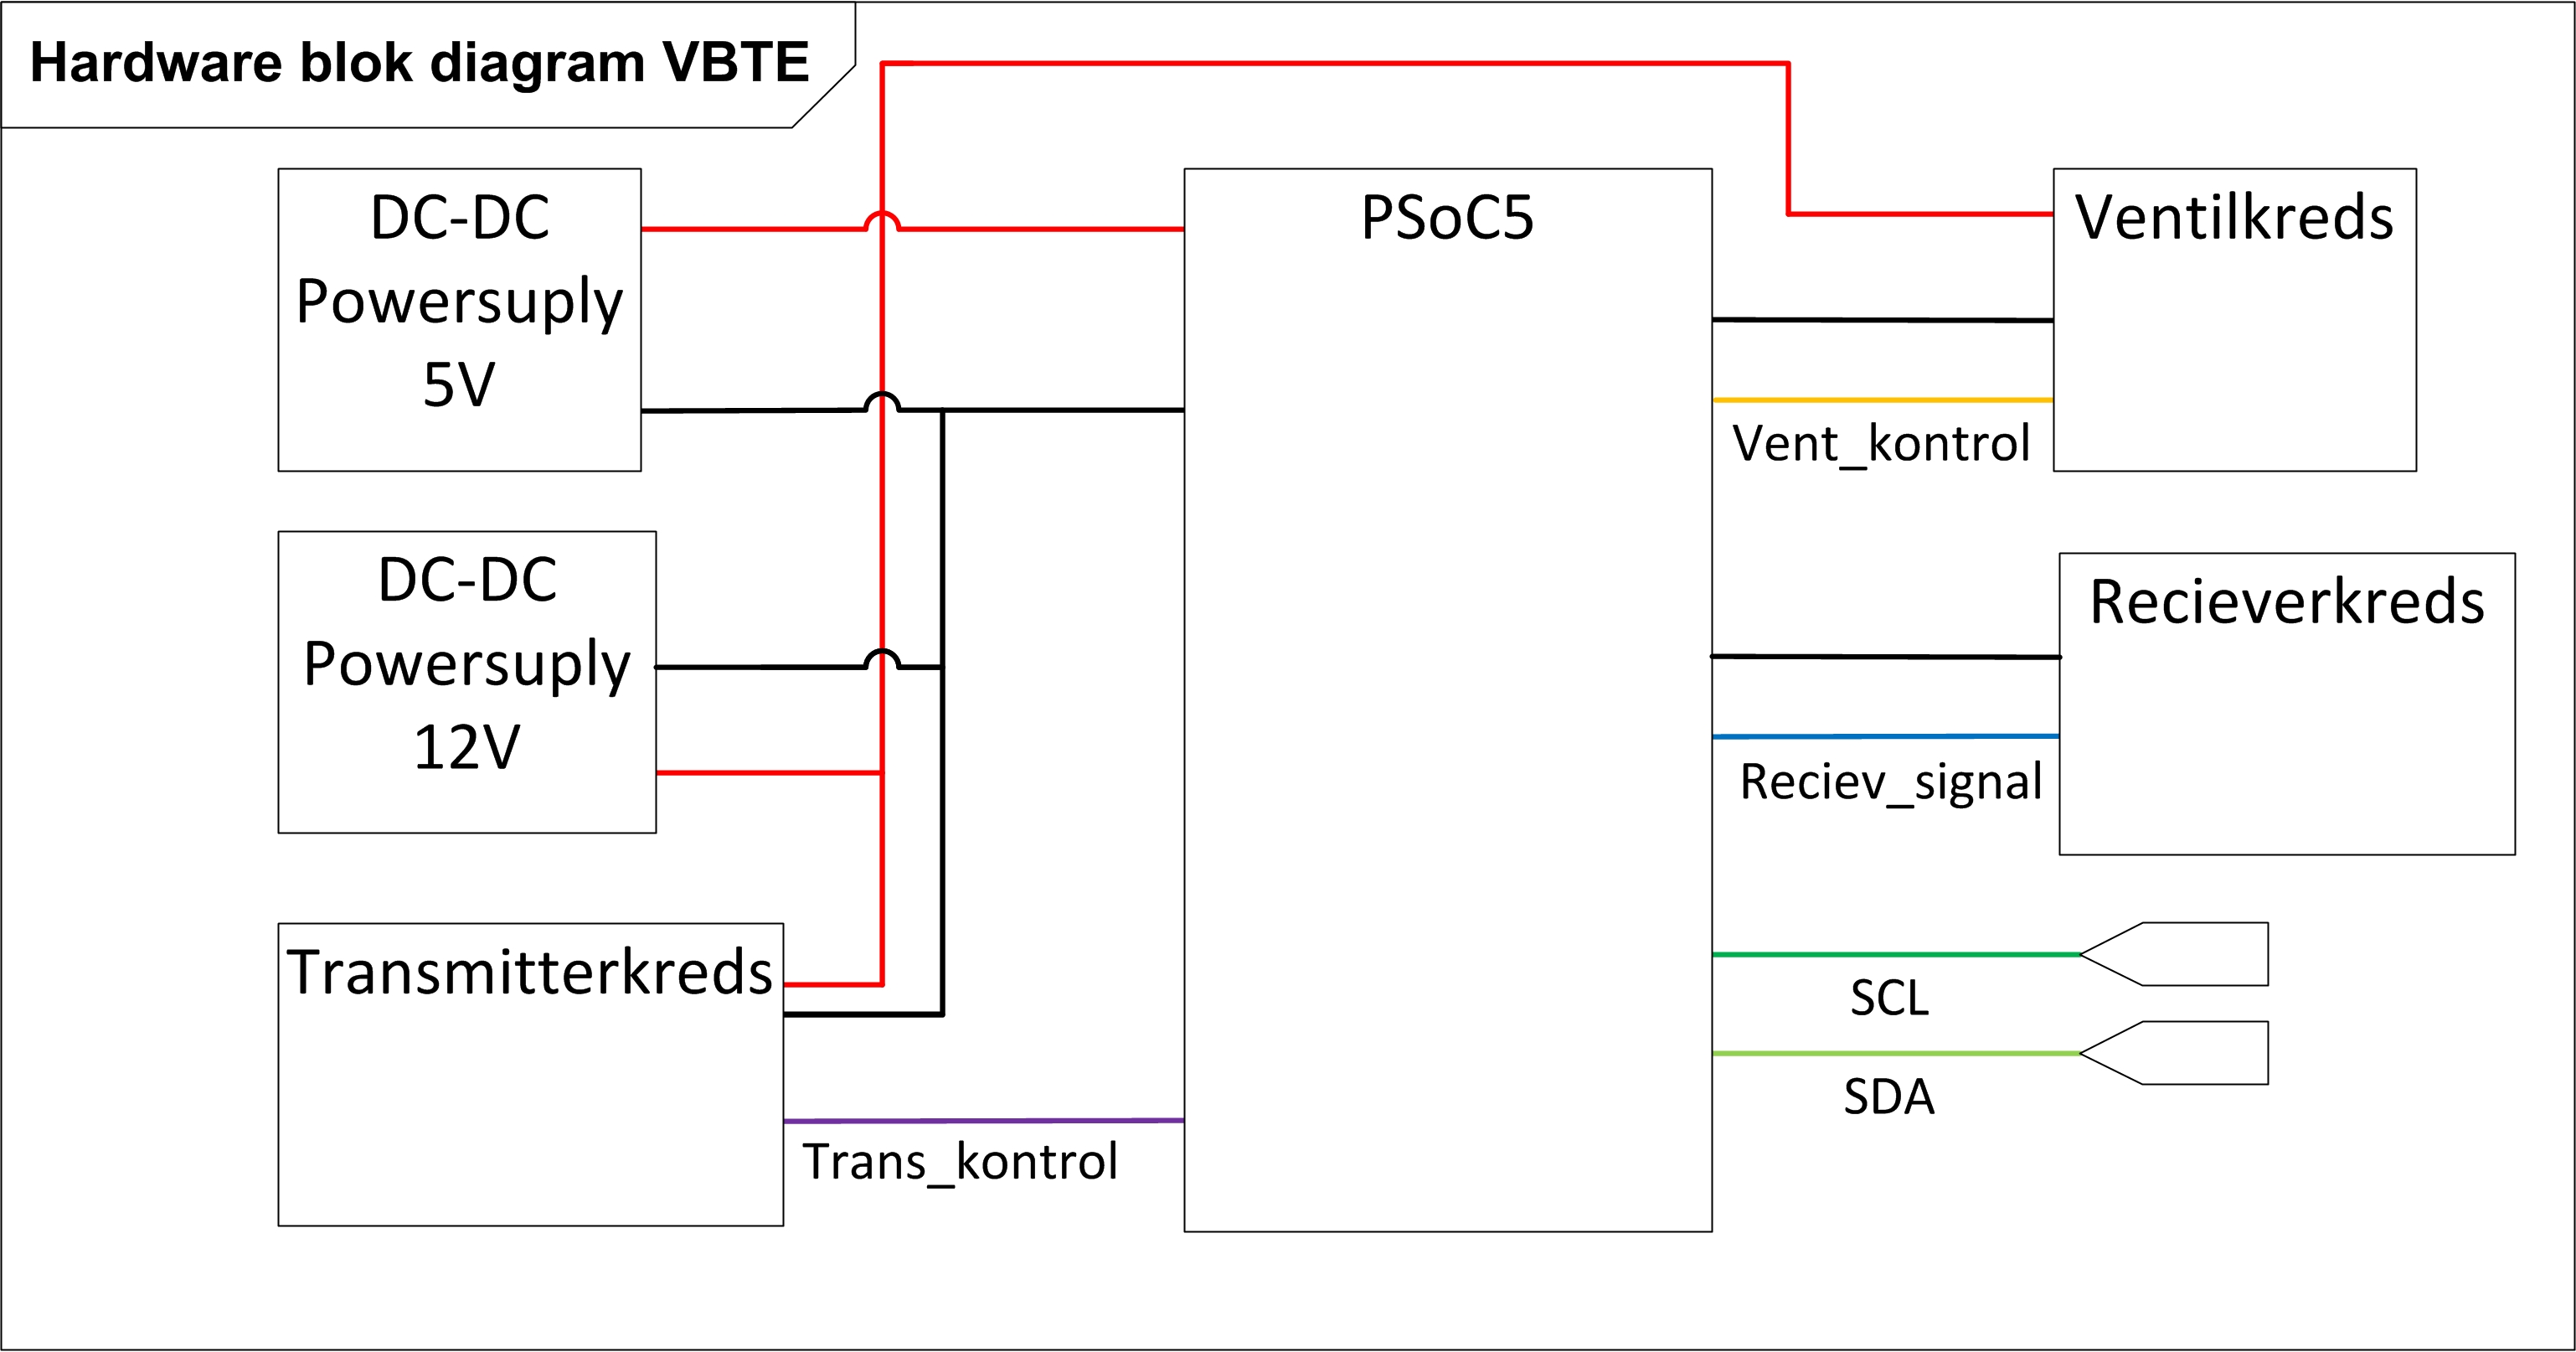
\includegraphics[width=.85\textwidth]{billeder/HWVBTE}
\caption{Overordnet blokdiagram for VBTE hardware}
\label{fig:HWVBTE}
\end{figure}
\subsection{Blokke}
Nedenfor beskrives de enkelte blokke illustreret på \textit{Figur~\ref{fig:HWVBTE}}
\subsubsection{PSoC5}
PSoC'en er den centrale del af VBTE'en og står for styringen af hele VBTE'en. Den består af:
\begin{itemize}
\item MicroController
\item PGA
\item Mixer
\item Timer
\item Clocks
\item I2C
\item Delta-Sigma ADC
\item Kontrolregister
\end{itemize}
PSoC'en er et færdigkøbt produkt og for detaljer om de enkelte blokke heri henvises der til databladet for PSoC5.
\subsubsection{DC-DC powersuply 5V}
Se powersuply afsnittet.
\subsubsection{DC-DC powersuply 12V}
Se powersuply afsnittet.
\subsubsection{Transmitterkreds}
Transmitterkredsen består af en MOSFET samt en keramisk ultralyds transmitter(Model: 400ST). Kredsen bliver drevet af 12V powersuply. \fxnote{Skal ligge i opbygningen af blokken i stedet for her}
\subsubsection{Reciverkreds}
Recierkredsen består af en keramisk ultralyds reciver(Model: 400SR).
\subsubsection{Ventilkreds}
Ventilkredsen består af en MOSFET samt en ventil(Model: EV210A-1.2 og EV210A-4.5)
\newpage
\section{Nedbrydning af blokke}
Nedenfor følger nedbrydningen af de enkelte blokke med henblik på at designe de enkelte dele til systemet. Nedbrydningen sker for at gøre designet nemmere og mere overskueligt.
\subsection{PSoC5}
På \textit{Figur \ref{fig:PSoCBlok}} ses HW-designet internt på PSoC'en. De enkelte blokke bliver beskrevet efterfølgende.
\begin{figure}[H]
\centering
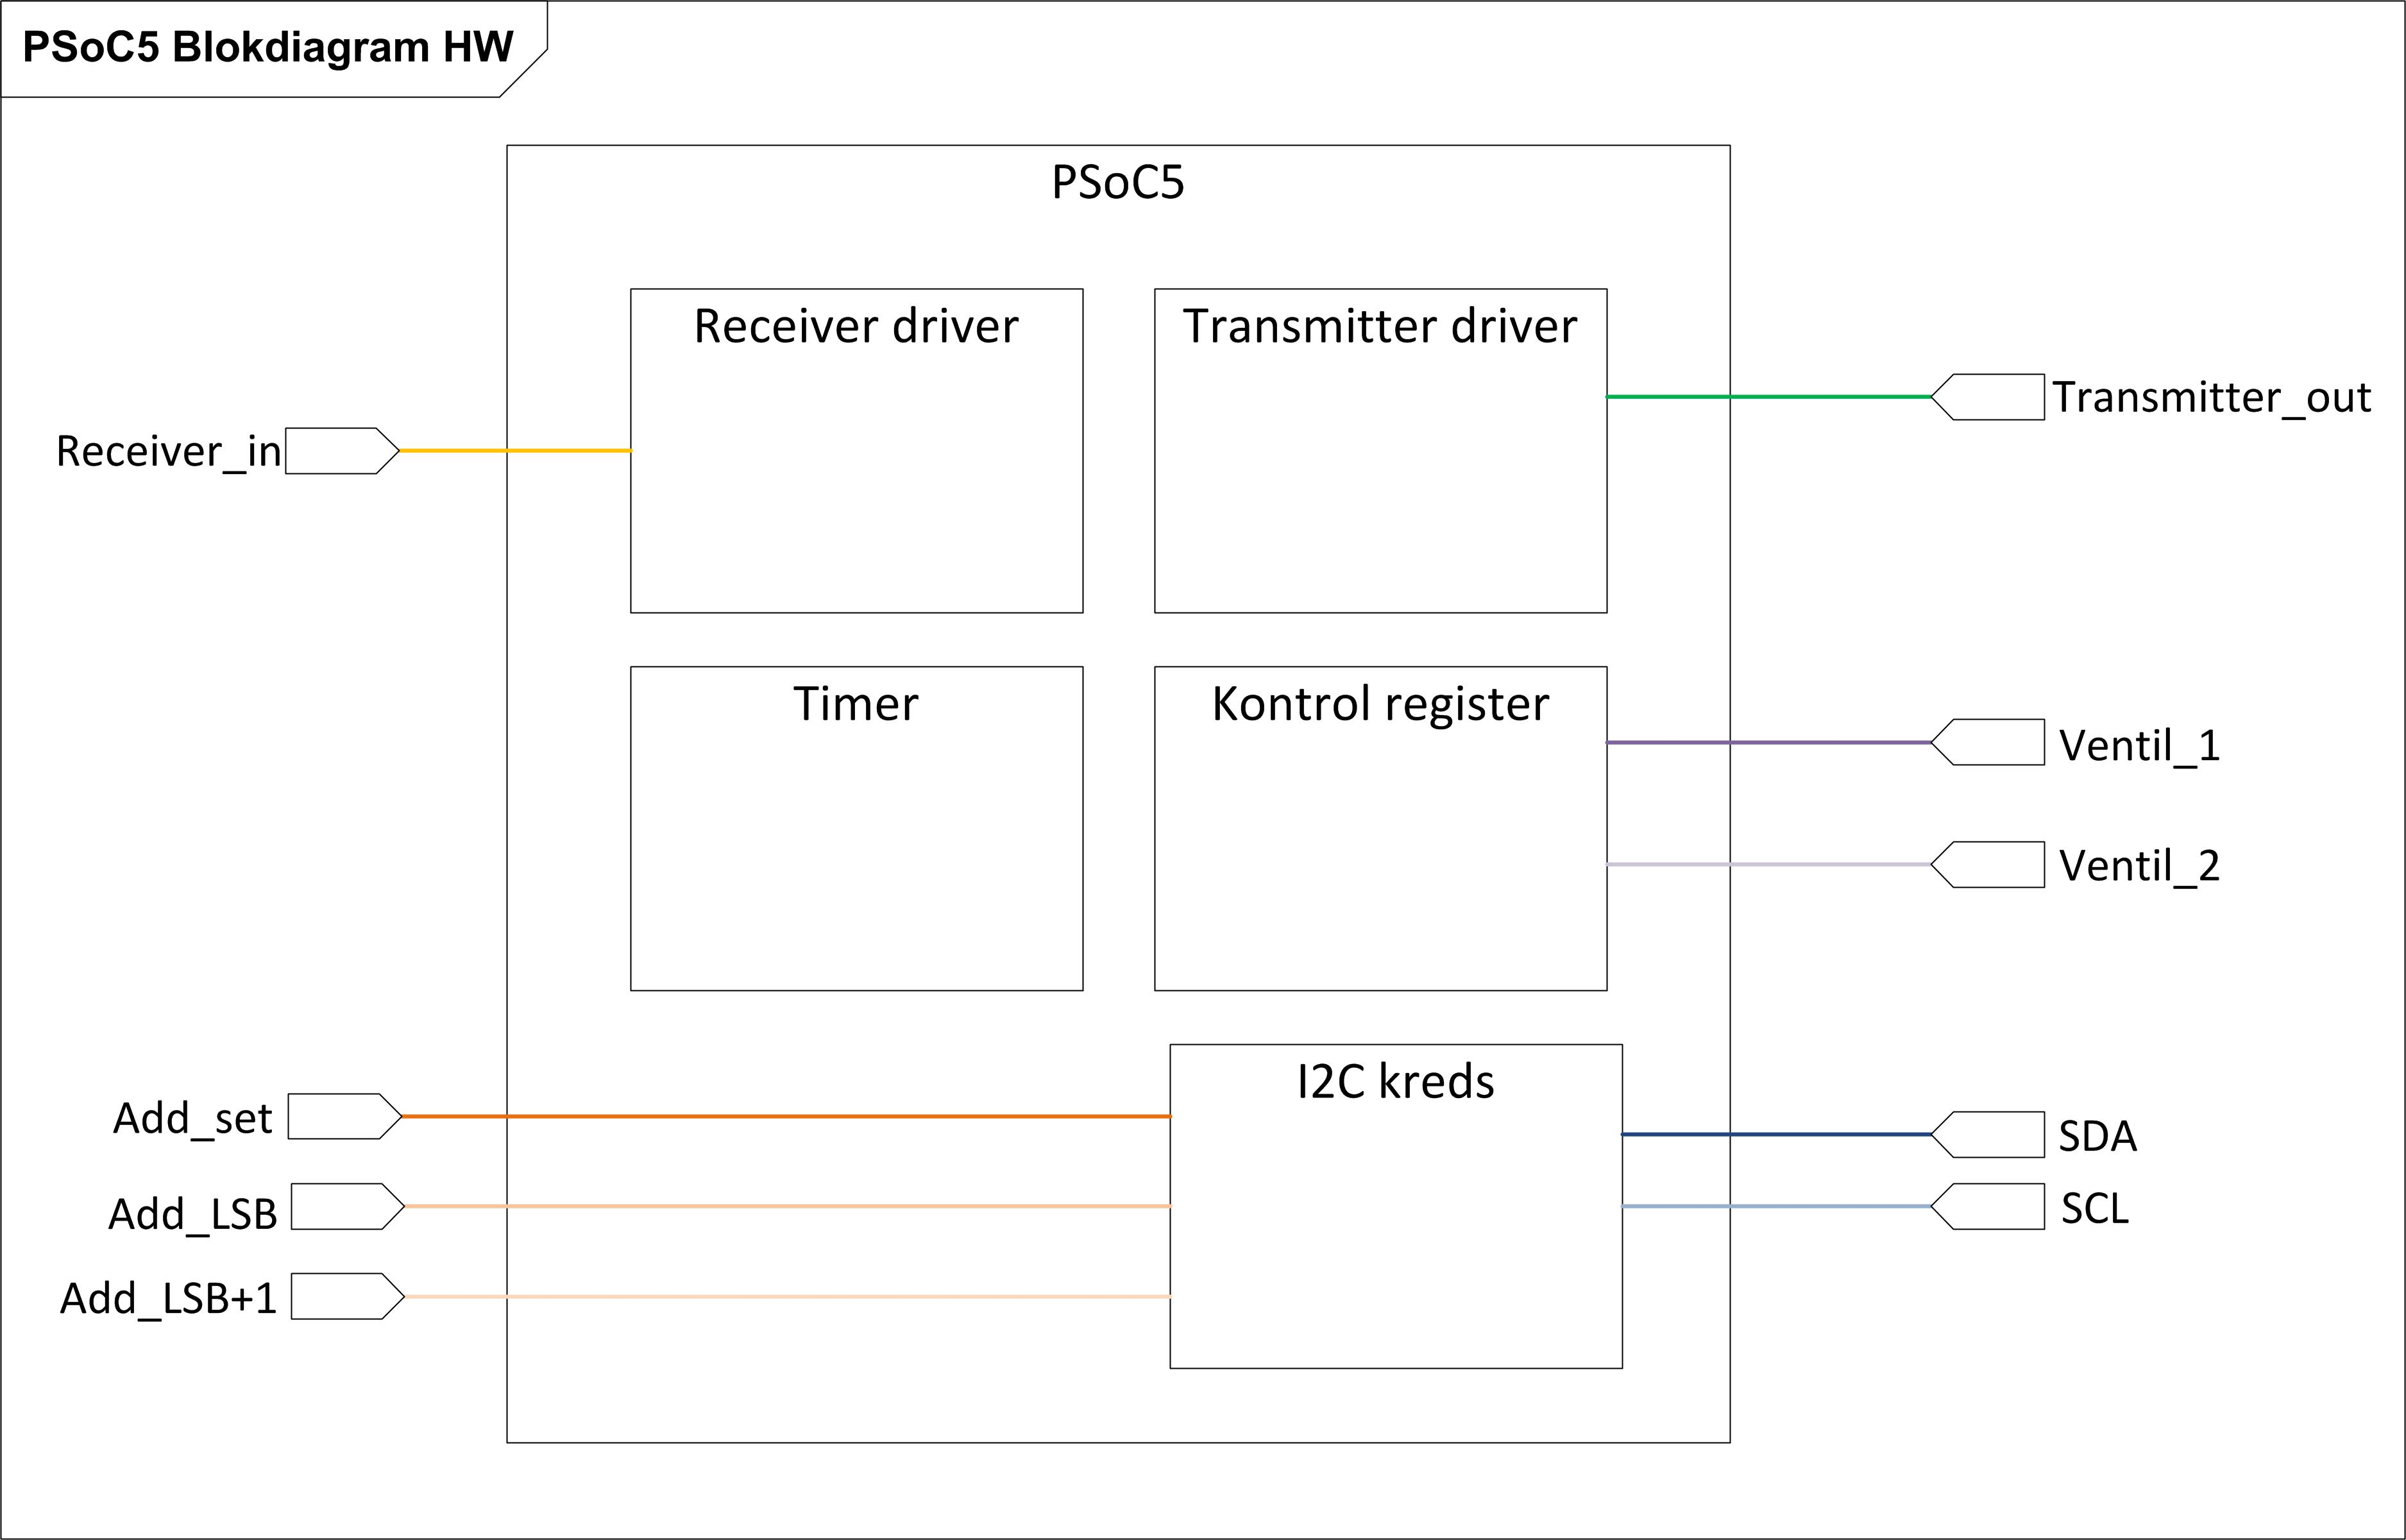
\includegraphics[width=.85\textwidth]{billeder/PSoCBlock}
\caption{PSoC5 blokdiagram}
\label{fig:PSoCBlok}
\end{figure}
\subsubsection{Signalbeskrivelser}
\begin{tabular}{|p{3cm}|p{3cm}|p{3cm}|p{4.5cm}|} \hline
\cellcolor[gray]{0.85}Signal navn& \cellcolor[gray]{0.85}Type &\cellcolor[gray]{0.85}Spænding&\cellcolor[gray]{0.85}Beskrivelse\\ \hline
Receiver\_in & Analog (AC = 40kHz) & Ligger fra ca 0.01V til 0.3V & Spænding genereret i ultralydsreceiveren.\\ \hline
Transmitter\_out & Analogt (AC = 40kHz) & ~0V til ~5V & Signal der skal styre ultralydstransmitteren \\ \hline
Vent\_1 & Digitalt & ~0V til ~5V & Signal der skal styre ventilen til at lukke vand ind med.\\ \hline
Vent\_2 & Digitalt & ~0V til ~5V & Signal der skal styre ventilen til at lukke vand ud med.\\ \hline
SDA & Digitalt & ~0V til ~5V & Et digitalt signal mellem VBTE og SM hvor I2C data læses fra.\\ \hline
SCL & Digitalt & ~0V til ~5V & Digitalt clocksignal til I2C.\\ \hline
Add\_set & Digitalt & ~0V til ~5V & Digitalt signal til at sætte I2C adressen. \\ \hline
Add\_LSB & Digitalt & ~0V til ~5V & Digitalt signal til at sætte LSB i I2C adressen. \\ \hline
Add\_LSB+1 & Digitalt & ~0V til ~5V & Digitalt signal til at sætte LSB i I2C adressen.\\ \hline



\end{tabular}\\
\textit{her skal der være en tabel med signalerne og deres spændingsniveauer og hvad de bærer af data}
\subsubsection{Timer}
Beskrivelse af timerblokkens opgave.
\subsubsection{I2C kreds}
Beskrivelse af I2C blokkens opgave samt dets interface.
\subsubsection{LCD Driver}
Beskrivelse af LCD driverens opgave samt dets interface
\subsubsection{Receiver Driver}
Beskrivelse af Receiver driverens opgave samt dets interface
\subsubsection{Transmitter Driver}
Beskrivelse af Transmitter driverens opgave samt dets interface
\subsubsection{Kontrol register}
Beskrivelse af Kontrol registerets opgave samt dets interface.

\subsection{Transmitter kreds}

